\documentclass[tikz,border=2pt]{standalone}
\usepackage{amsmath,amssymb}
\usepackage{tikz}
\usetikzlibrary{arrows.meta}

\begin{document}
% Rank = dimension of the column space: independent columns span the plane (rank 2),
% proportional columns only a line (rank 1).
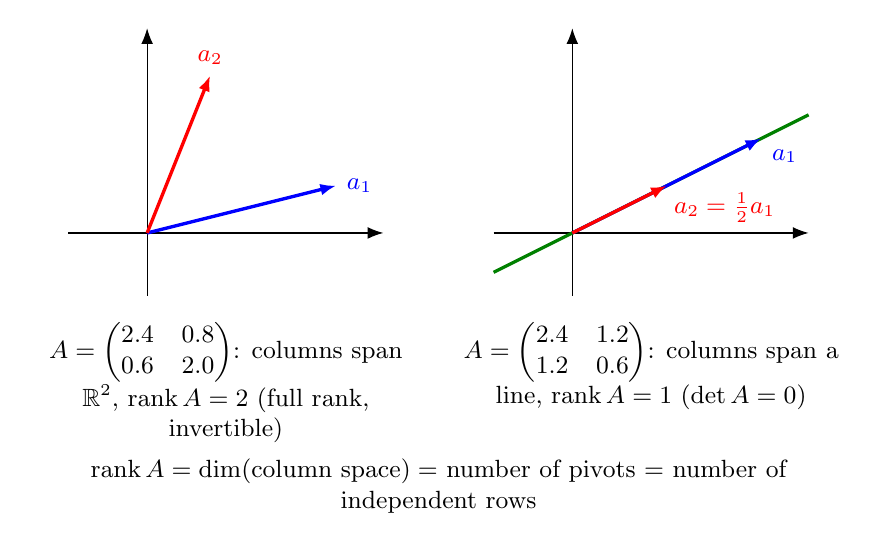
\begin{tikzpicture}[every node/.style={font=\small}, >={Latex[length=2mm]}]
	\begin{scope}
		\draw[->] (-1.0,0) -- (3.0,0);
		\draw[->] (0,-0.8) -- (0,2.6);
		\draw[->, blue, very thick] (0,0) -- (2.4,0.6) node[right] {$a_1$};
		\draw[->, red, very thick] (0,0) -- (0.8,2.0) node[above] {$a_2$};
		\node[anchor=north, align=flush center, text width=4.8cm] at (1,-1.0) {$A=\begin{pmatrix}2.4&0.8\\0.6&2.0\end{pmatrix}$: columns span $\mathbb{R}^2$, $\operatorname{rank}A=2$ (full rank, invertible)};
	\end{scope}
	\begin{scope}[xshift=5.4cm]
		\draw[->] (-1.0,0) -- (3.0,0);
		\draw[->] (0,-0.8) -- (0,2.6);
		\draw[green!50!black, very thick] (-1.0,-0.5) -- (3.0,1.5);
		\draw[->, blue, very thick] (0,0) -- (2.4,1.2) node[below right] {$a_1$};
		\draw[->, red, very thick] (0,0) -- (1.2,0.6) node[below right, inner sep=2pt] {$a_2=\tfrac12a_1$};
		\node[anchor=north, align=flush center, text width=4.8cm] at (1,-1.0) {$A=\begin{pmatrix}2.4&1.2\\1.2&0.6\end{pmatrix}$: columns span a line, $\operatorname{rank}A=1$ ($\det A=0$)};
	\end{scope}
	\node[anchor=north, align=flush center, text width=10cm] at (3.7,-2.75) {$\operatorname{rank}A=\dim(\text{column space})=$ number of pivots $=$ number of independent rows};
\end{tikzpicture}
\end{document}
